\section{Question 3} 
ISS spacecraft observation orbital elements and Ground Station Location location is provided in \ref{table:orbital-elements}, and \ref{table:lat-long}, respectively. The orbital elements are used to calculate the position of the ISS spacecraft at the time of observation. The position is then used to calculate the line of sight vector from the ground station to the ISS spacecraft. The line of sight vector is then used to calculate the elevation and azimuth angles of the ISS spacecraft. The elevation and azimuth angles are then used to calculate spacecraft visibility.
\begin{table}[H]
    \centering
    \label{table:orbital-elements}
    % \vspace{.2cm}
    \Tstrut
    \begin{tabular}{|c|c|}
    \hline
    Orbital Element & Value \\
    \hline
    Eccentricity & 0.0005771 \\
    Inclination & \ang{51.6409} \\
    Perigee Height & 415km \\
    Apogee Height & 423km \\
    RAAN & \ang{88.8414} \\
    Argument of Perigee & \ang{75.2083} \\
    True Anomaly & 0 \\
    \hline
    \end{tabular}
    \caption{ISS Observation}
\end{table}

\begin{figure}[H]
    \centering
    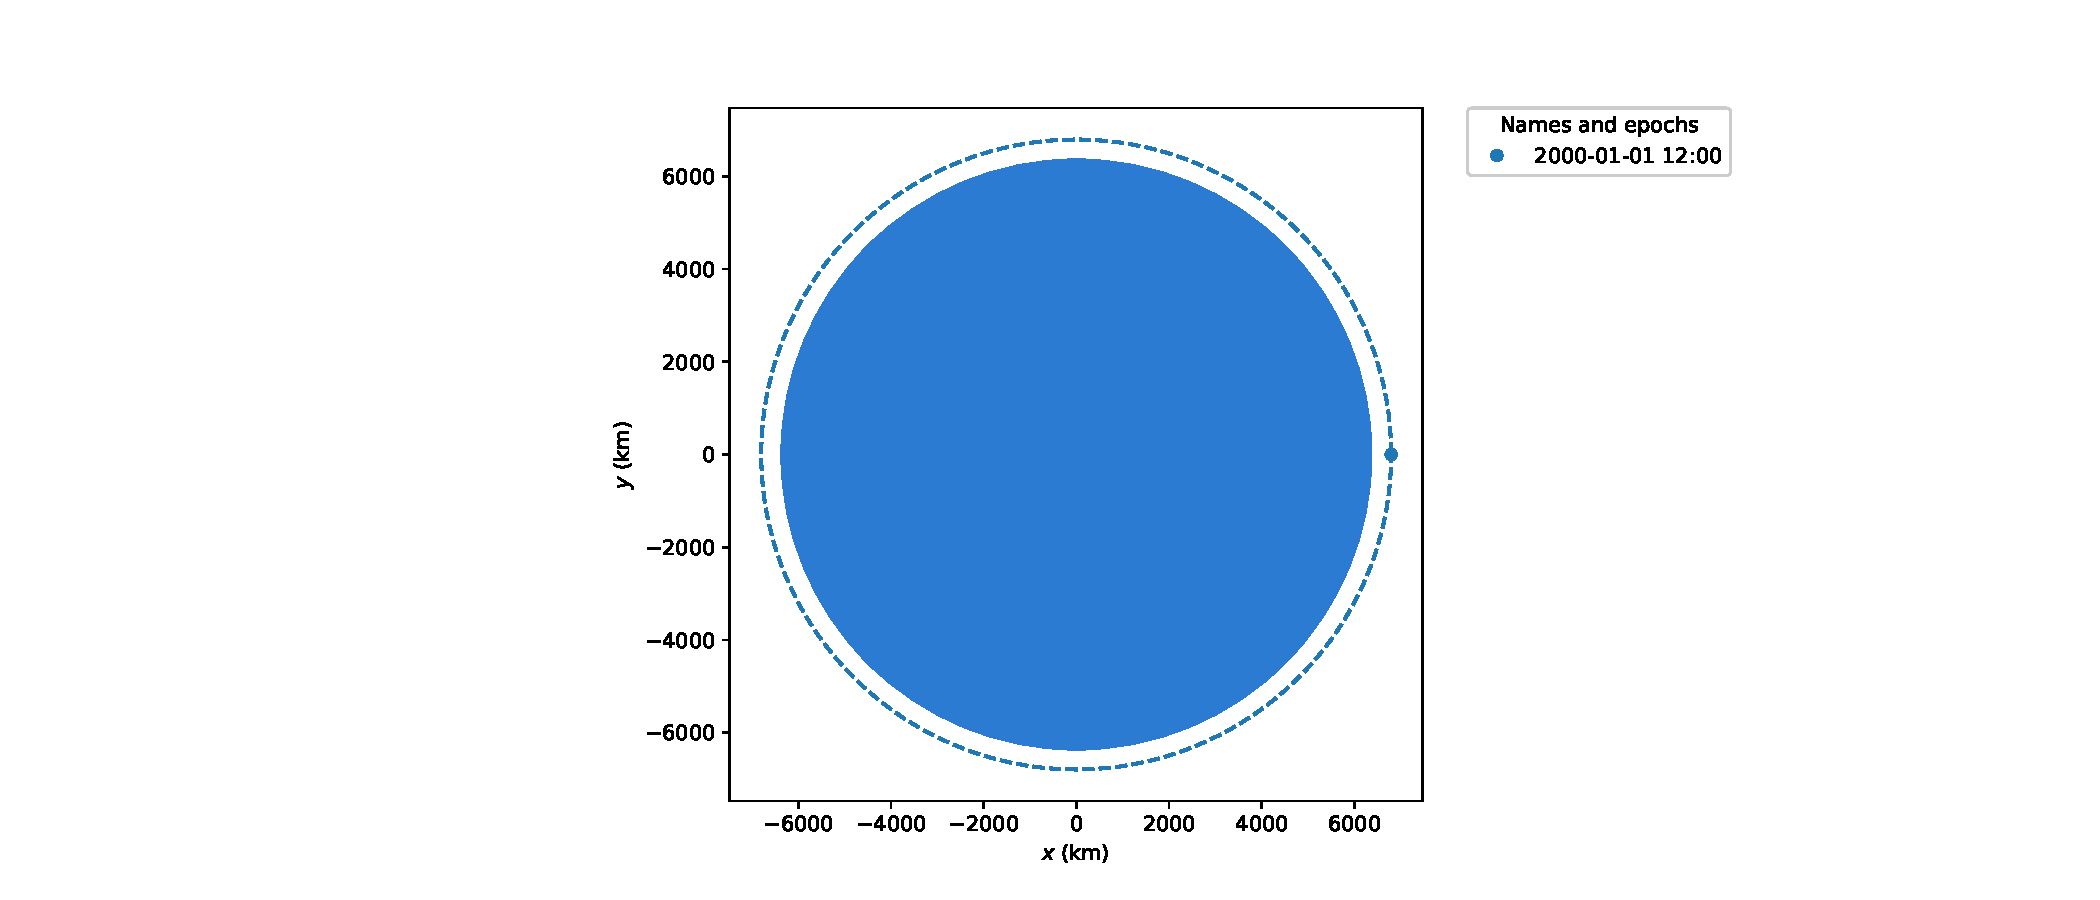
\includegraphics[width=1\textwidth]{../Figure/Q3/orbiral}
    \caption{ISS spacecraft orbit.}
    \label{fig:ISS_orbit}
\end{figure}

\begin{figure}[H]
    \centering
    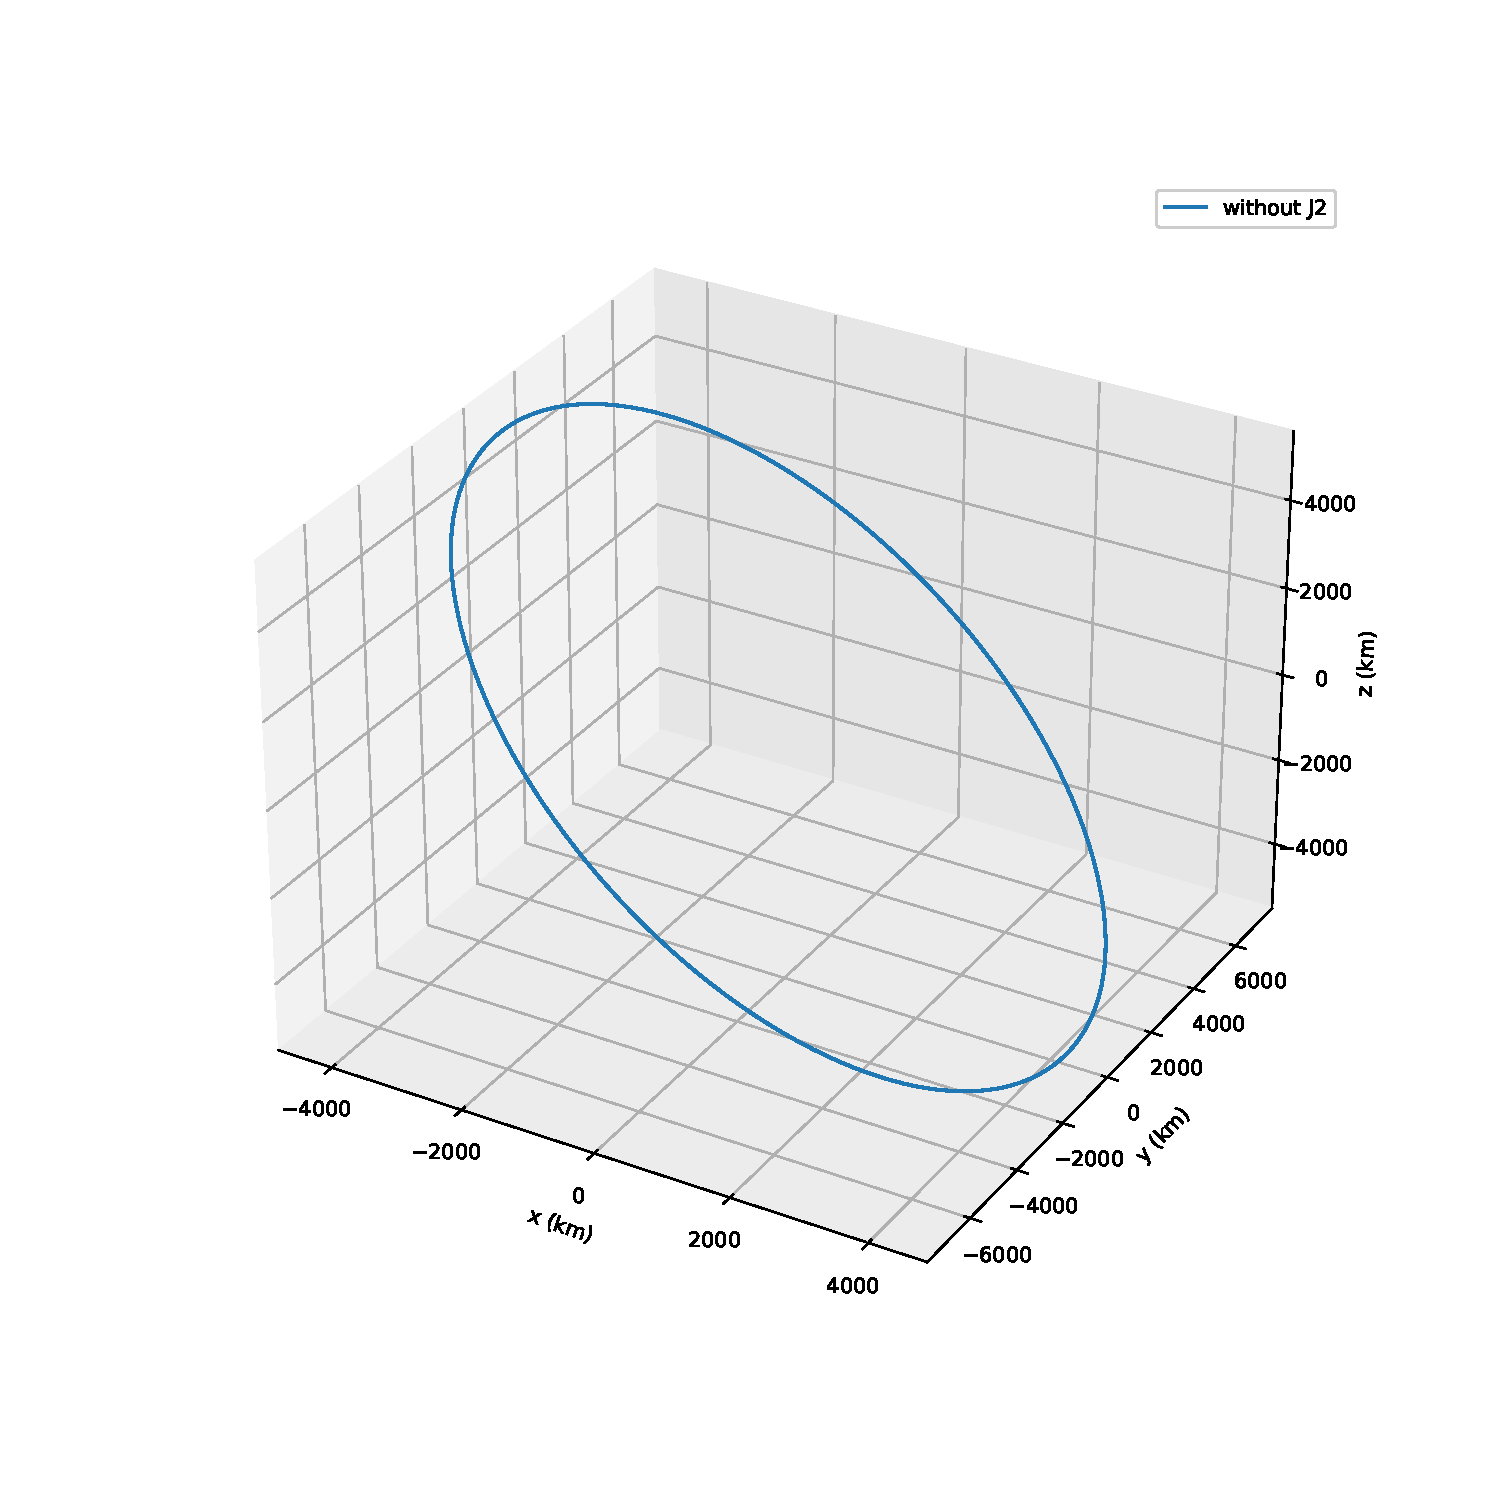
\includegraphics[width=1\textwidth]{../Figure/Q3/ISS_trajectory_no_per}
    \caption{ISS spacecraft orbit trajectory without perturbation}
\end{figure}
\subsection{$J_2$ perturbation}
In this section we add $J_2$ perturbation to the orbit of the ISS spacecraft. The $J_2$ perturbation is added to the ISS spacecraft orbit by adding the $J_2$ perturbation to the mean motion of the ISS spacecraft. The $J_2$ perturbation is calculated using the following equation:
\begin{equation}
    \begin{aligned}
        \ddot{x} &= -\frac{\mu}{r^3}x + \frac{3}{2} \frac{J_2 \mu R^2}{r^4} \left( 1 - 5 \frac{z^2}{r^2} \right) x \\
        \ddot{y} &= -\frac{\mu}{r^3}y + \frac{3}{2} \frac{J_2 \mu R^2}{r^4} \left( 1 - 5 \frac{z^2}{r^2} \right) y \\
        \ddot{z} &= -\frac{\mu}{r^3}z + \frac{3}{2} \frac{J_2 \mu R^2}{r^4} \left( 3 - 5 \frac{z^2}{r^2} \right) z \\
    \end{aligned}
\end{equation}

ISS trajectory is shown in below figure.
\begin{figure}[H]
    \centering
    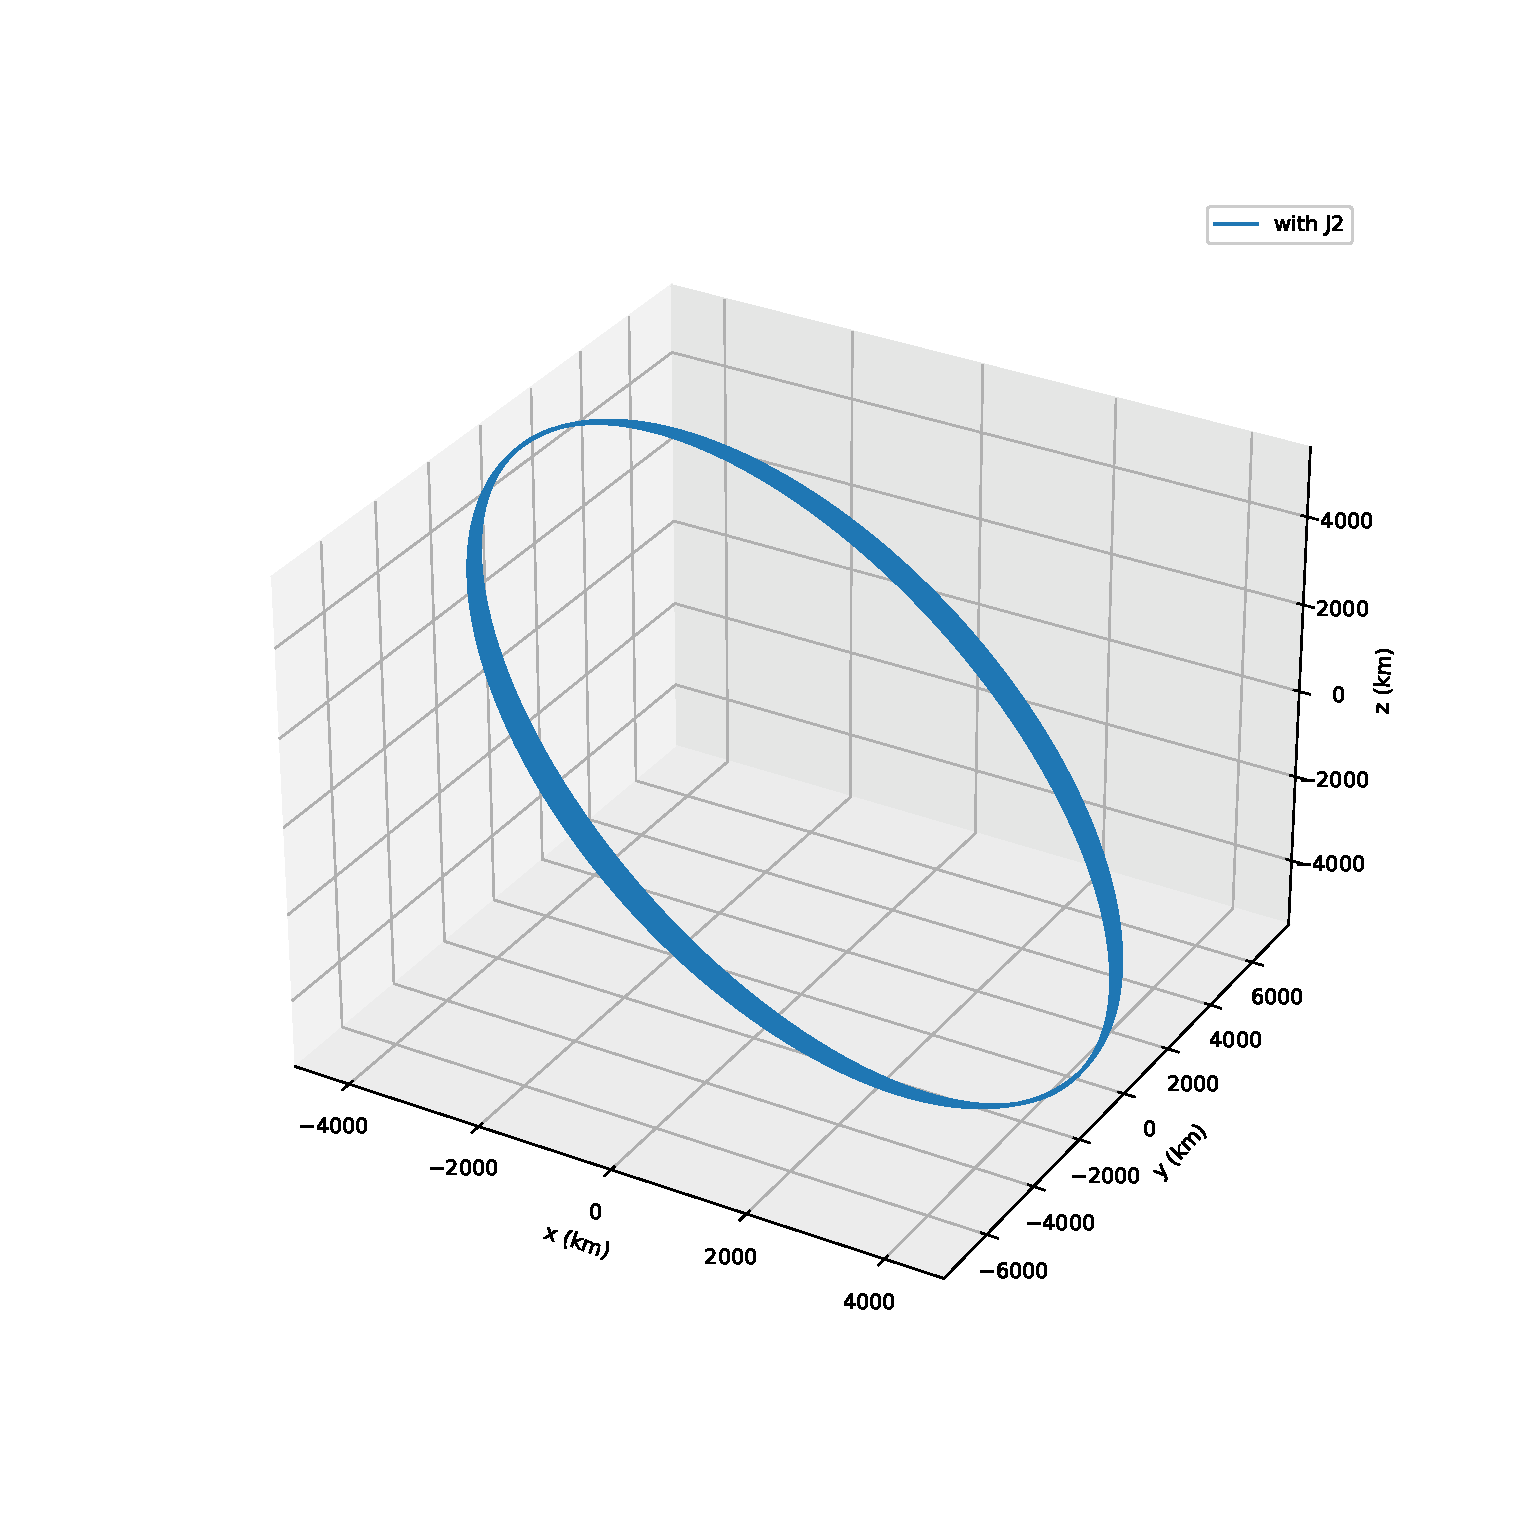
\includegraphics[width=1\textwidth]{../Figure/Q3/ISS_trajectory_J2}
    \caption{ISS spacecraft orbit trajectory with $J_2$ perturbation}
\end{figure}

\subsection{Study difference $J_2$ perturbation orbital}
In this section, we study $J_2$ perturbation in trajectory and error that make with ideal trajectory.

\begin{figure}[H]
    \centering
    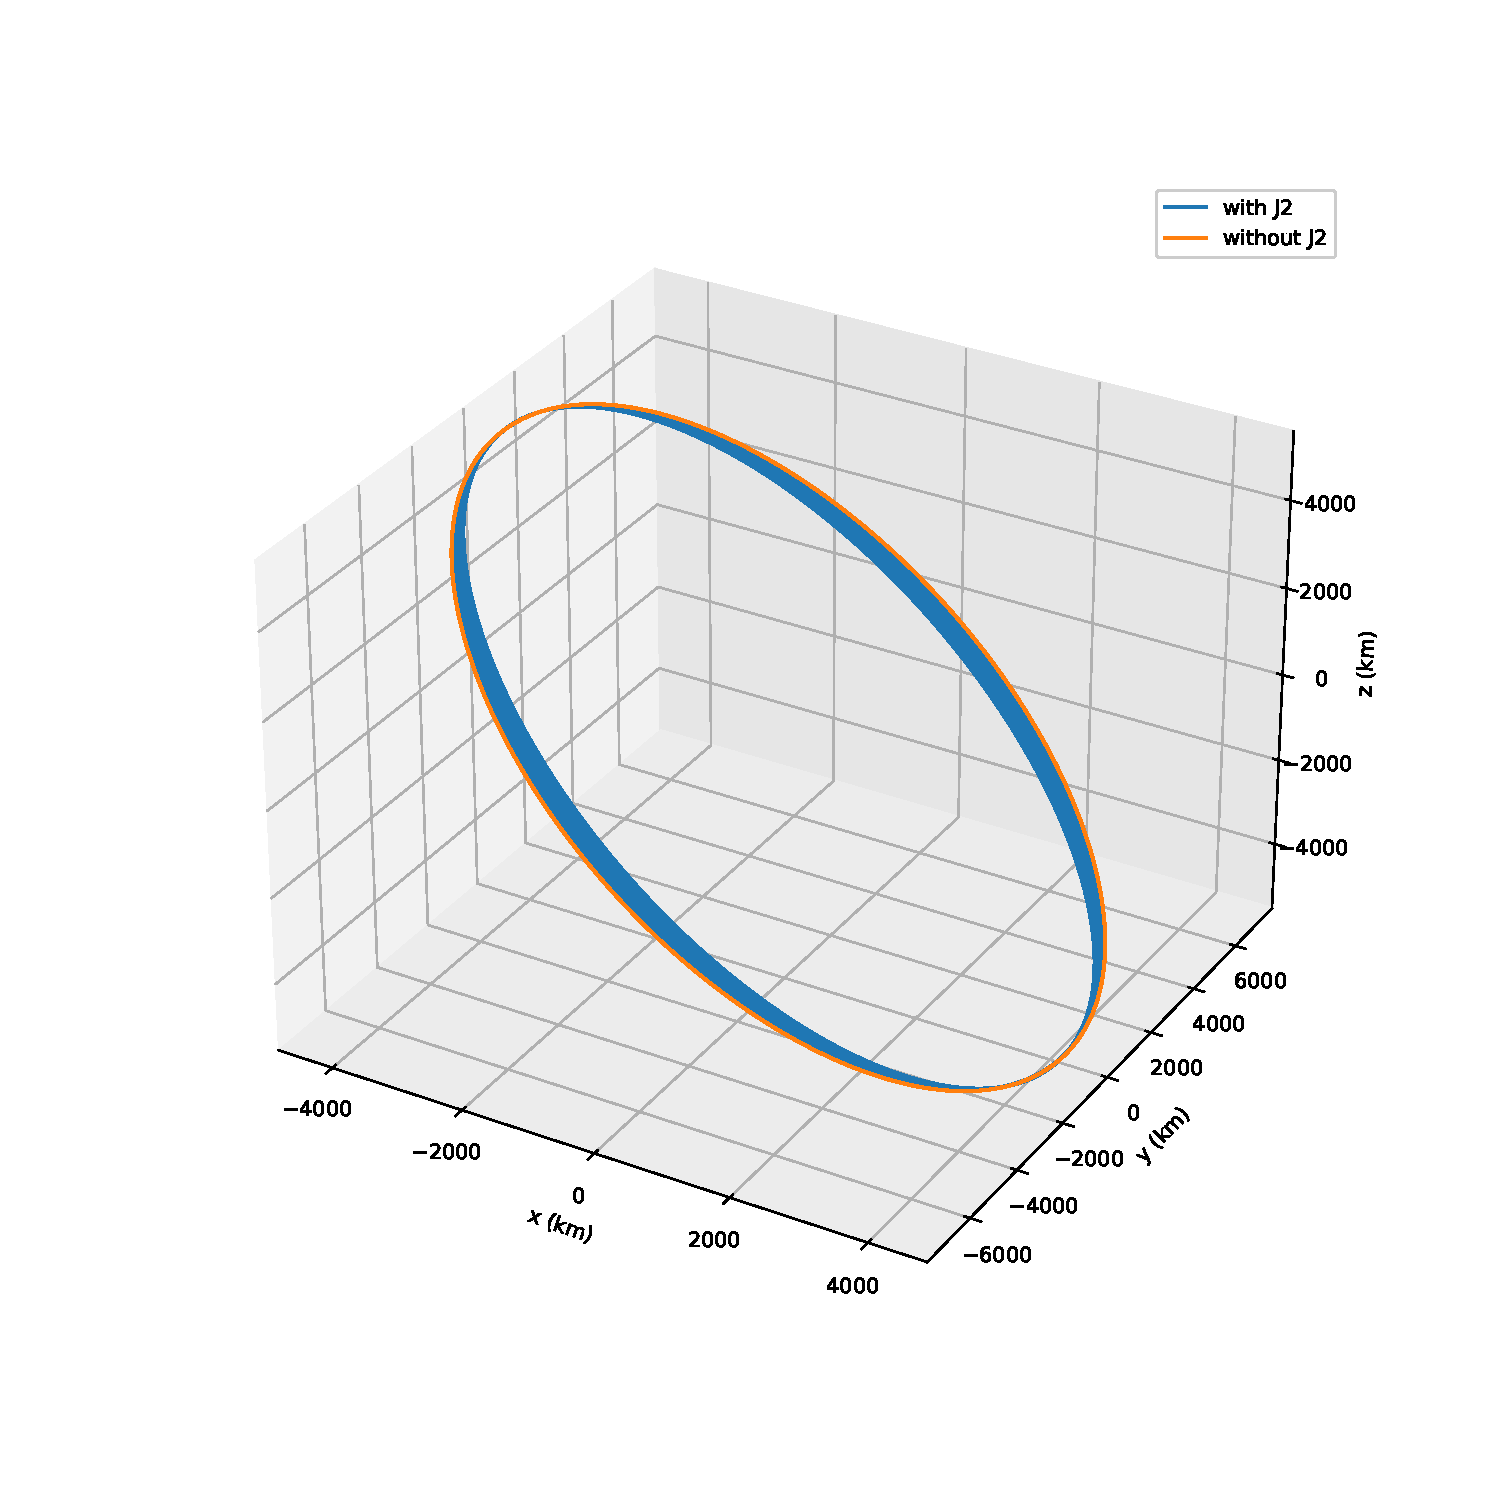
\includegraphics[width=1\textwidth]{../Figure/Q3/ISS_trajectory}
    \caption{$J_2$ perturbation effect on ISS spacecraft orbit trajectory}
\end{figure}
Below figures show error vector with function of time.

\begin{figure}[H]
    \centering
    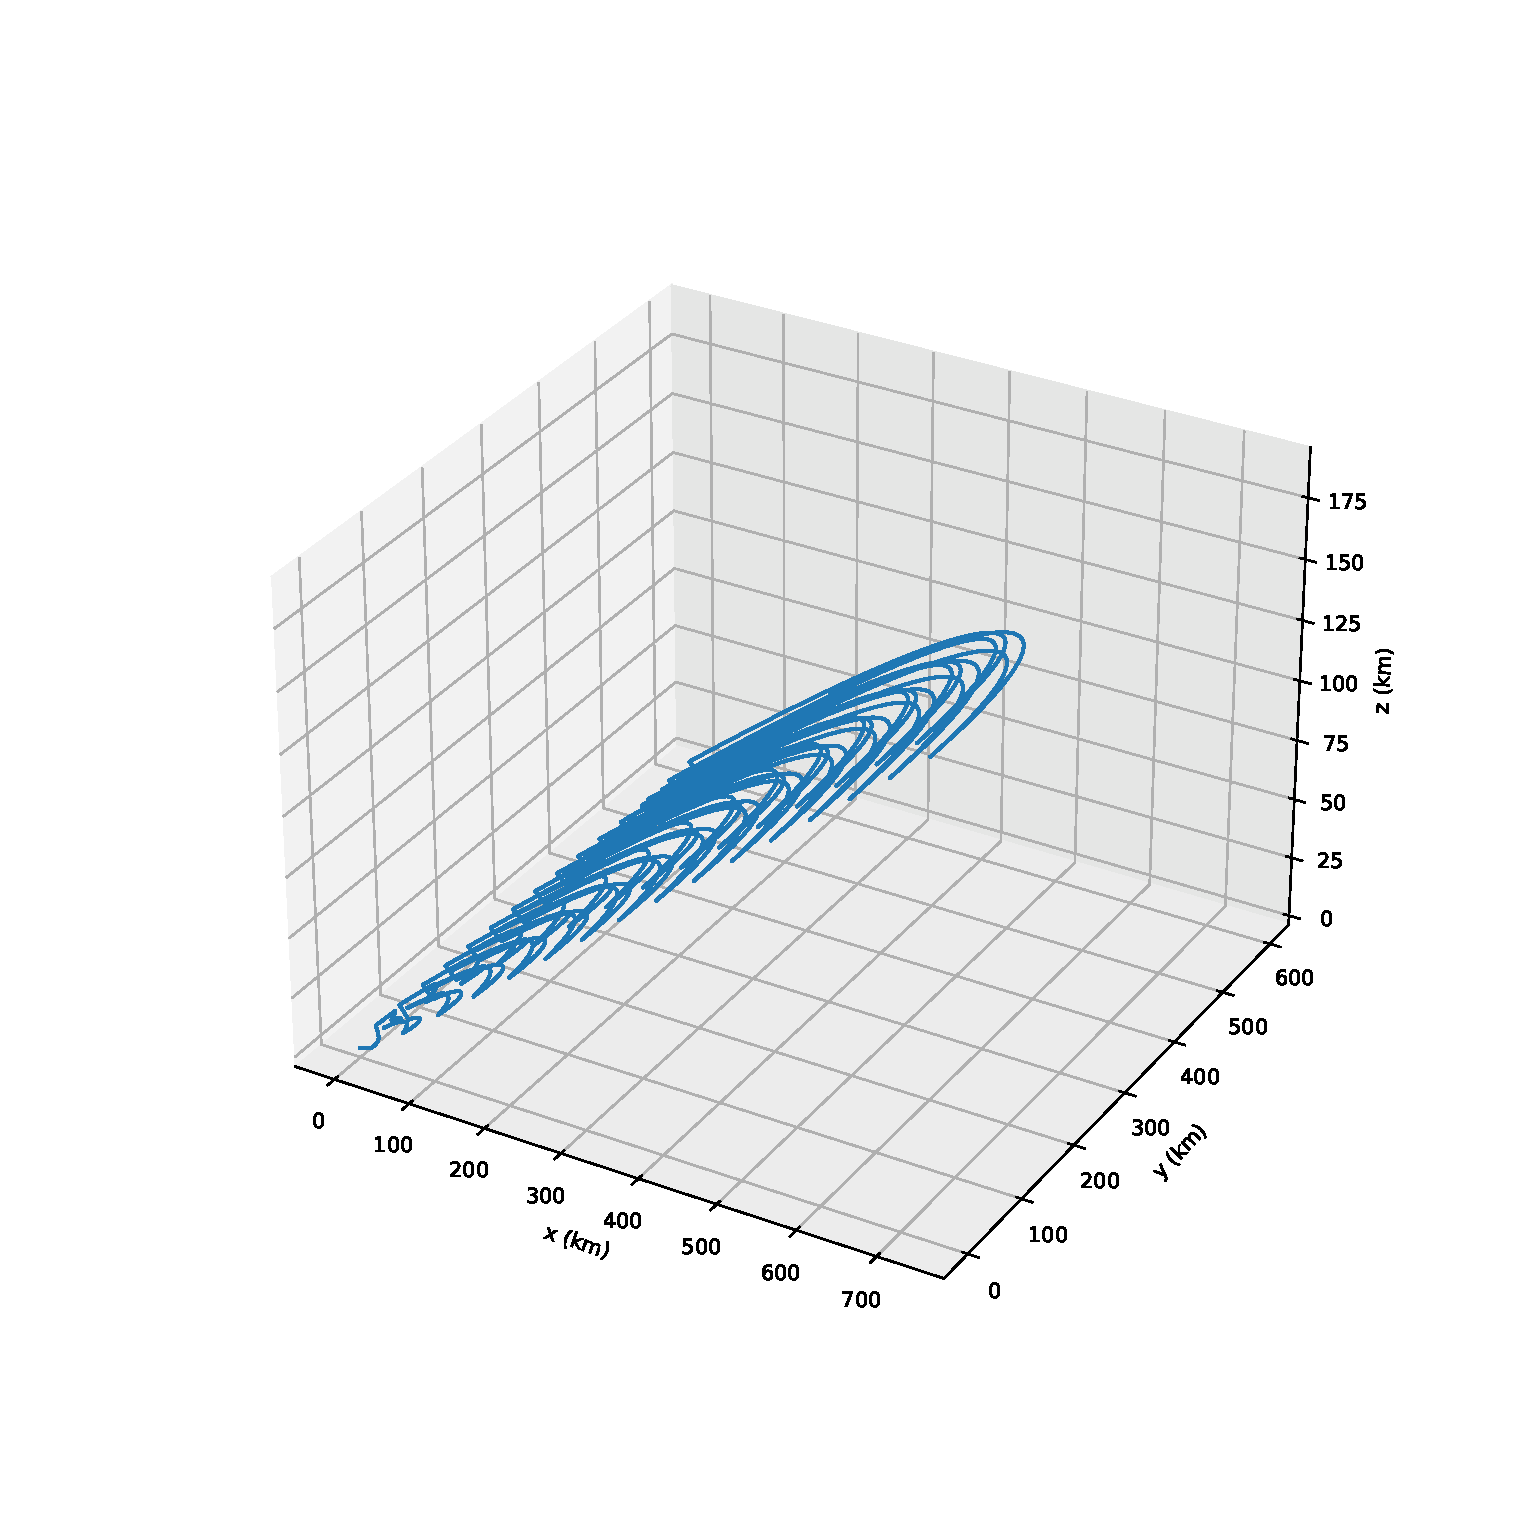
\includegraphics[width=1\textwidth]{../Figure/Q3/ISS_trajectory_error_3D}
    \caption{$J_2$ perturbation error vector with ideal trajectory}
\end{figure}

\begin{figure}[H]
    \centering
    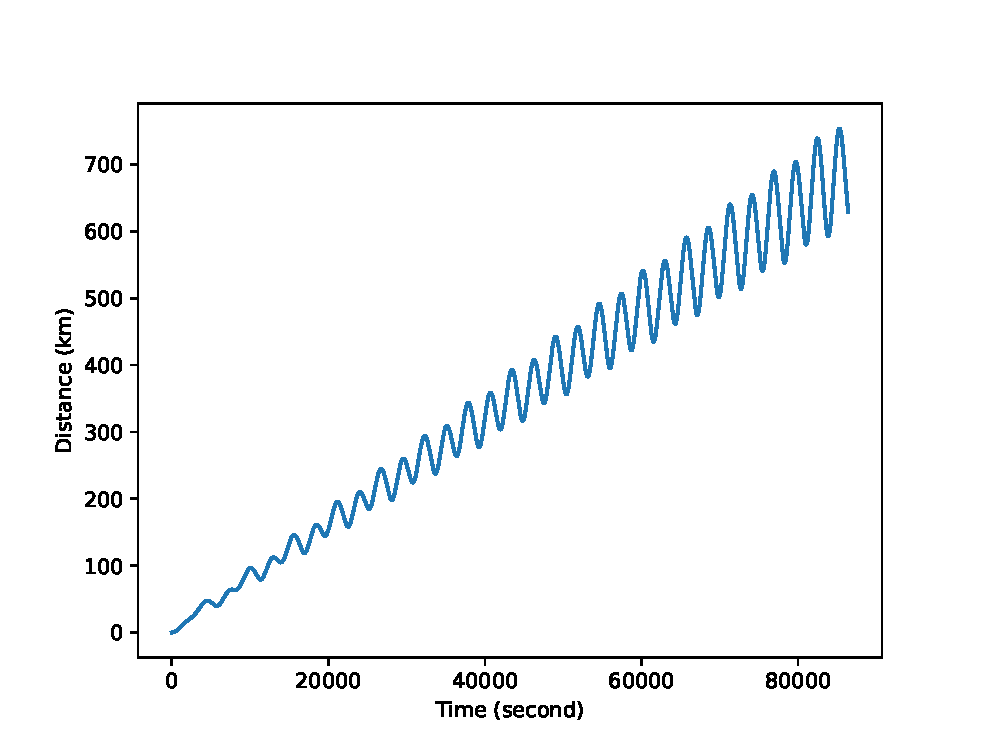
\includegraphics[width=1\textwidth]{../Figure/Q3/ISS_trajectory_error_all}
    \caption{$J_2$ perturbation error with ideal trajectory}
\end{figure}


\subsection{Allowable error}
In the previous part, we see the error but its magnitude is larger than 180 m and we can't see when the error is 180 meters. The below figure shows less time for simulation and finding when the error is 180 meters, and it's about 140 seconds.

\begin{figure}[H]
    \centering
    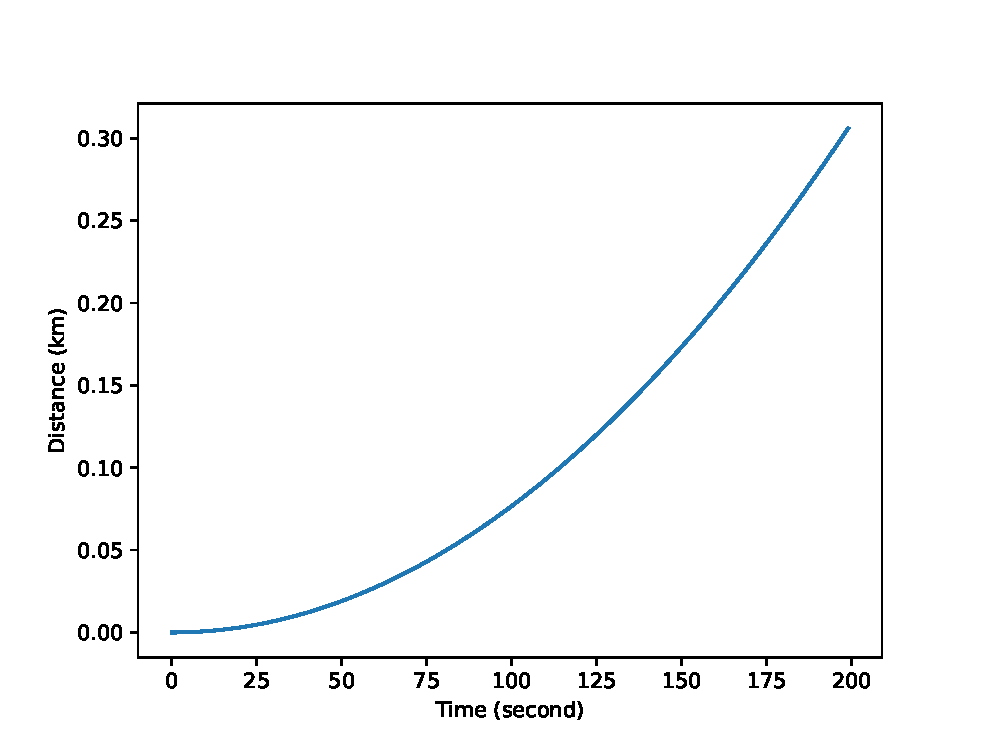
\includegraphics[width=1\textwidth]{../Figure/Q3/ISS_trajectory_error_min}
    \caption{$J_2$ perturbation error with ideal trajectory till 200 seconds}
\end{figure}